\documentclass[utf8]{beamer}
\mode<presentation>
\usepackage[spanish]{babel}
\usepackage{multicol}
\useoutertheme{infolines} 
\usepackage{graphicx}
\usetheme{boxes}

\definecolor{lightblue}{rgb}{0,.5,1}
%\beamertemplateshadingbackground{lightblue!50}{lightblue!50}
%\setbeamercovered{transparent}


\begin{document}
\usebackgroundtemplate{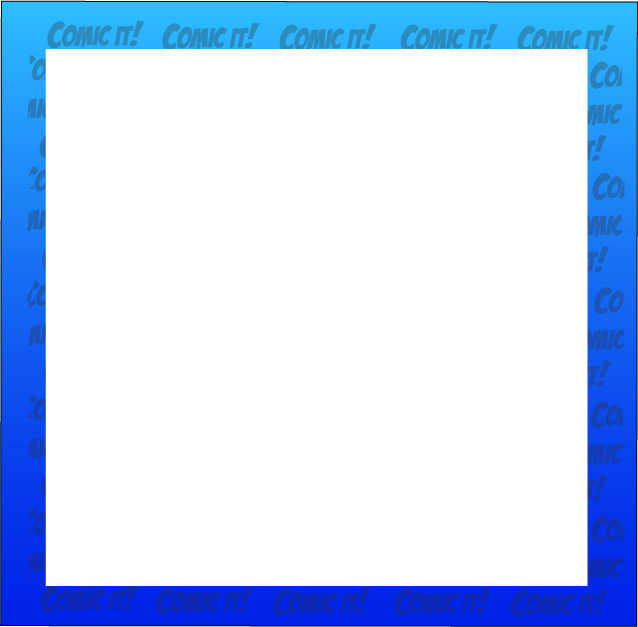
\includegraphics[width= \paperwidth, height=\paperheight]{fondoazul.jpg}}
	\begin{frame}	
		\color{red}\textbf{\begin{center}{\Huge{¡Creando Historietas!}}\end{center}}				
		\pause
		\begin{center} 
				 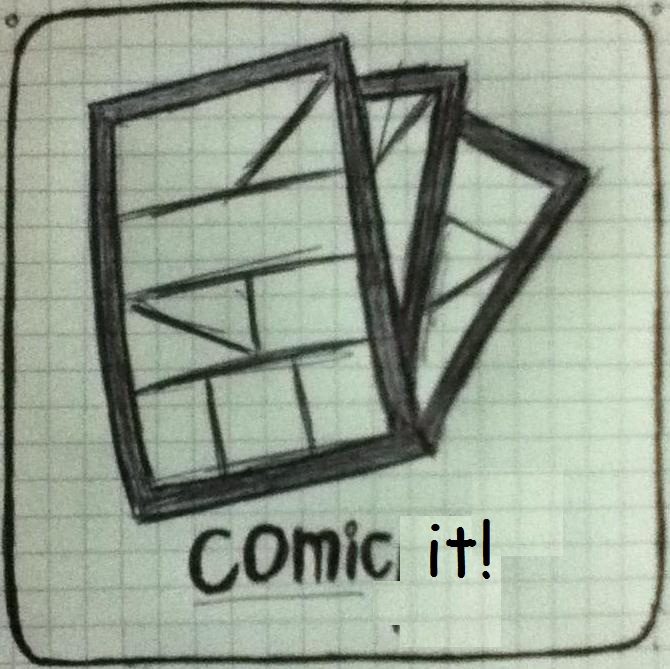
\includegraphics[width=0.5\textwidth]{comicit.jpg} %Midifico el width para cambiar el tamaño%
		\end{center}
	\end{frame}
\usebackgroundtemplate{
\includegraphics[width= \paperwidth, height=\paperheight]{fondoaz.jpg}}
	\begin{frame}	 	
		\color{red}\textbf{\begin{center}{\Huge{Autores}}\end{center}}
		\color{black}
		\begin{center}\huge{ 
			\pause
			- Ana Arias\\
			\pause
			- Liliana Ramos\\
			\pause
			- Denny Schuldt
			
			\pause
		}
			\normalsize
			\vspace{9mm}
			 Lenguajes de Programación
			\\2012 - II Término			
		\end{center}				
	\end{frame}
	\begin{frame}
		\begin{center} 
			 
\includegraphics[width=0.8\textwidth]{funcionalidades.jpg}
		\end{center}
	\end{frame}
	\begin{frame}
		\frametitle{
	 		\begingroup
				\begin{center}
					\normalsize
					\color{blue}Utiliza imágenes de tu librería...
					\pause
					\newline
					 ¡Crea tu propia historieta!
					\pause
				\end{center}
			\endgroup
		}
		\begin{center}
			\begin{itemize}
				\vspace{-1cm}
				\item\textbf{PLANTILLAS PARA COLOCAR LAS IMAGENES EN LA HISTORIETA:}
				\newline
				El usuario podrá escoger la plantilla con la cual empezar su comic!
			\end{itemize}
		\end{center}
		\begin{center} 
			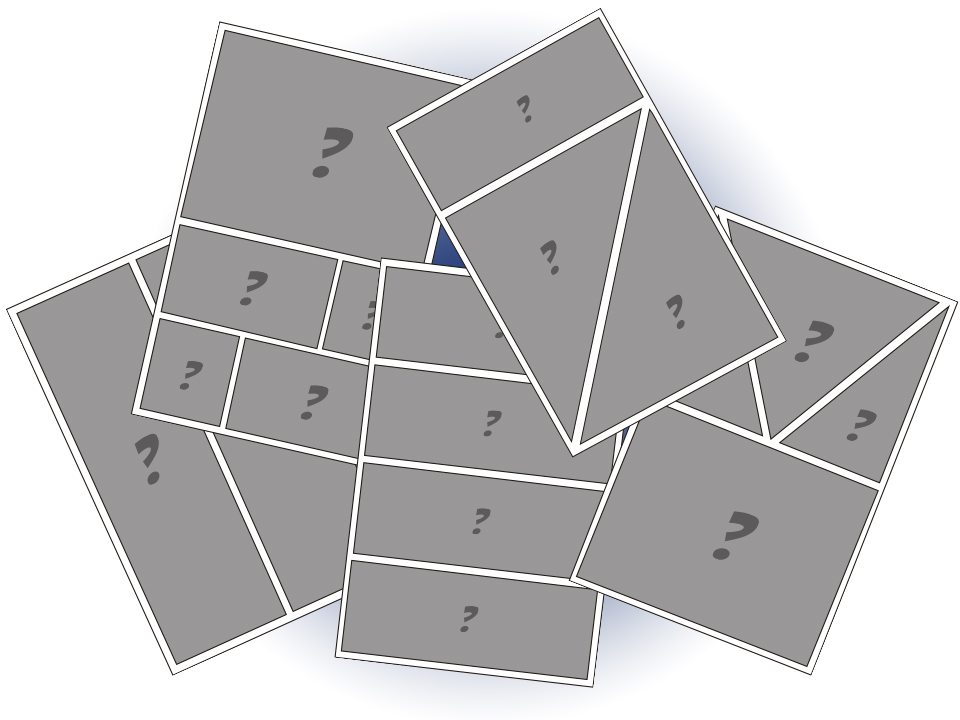
\includegraphics[width=0.4\textwidth]{plantillas.jpg}
		\end{center}
	\end{frame}
	\begin{frame}
		\frametitle{
	 		\begingroup
				\begin{center}
				\normalsize
				\color{blue}¡Crea el diálogo de tus personajes!
				\pause
				\end{center}
			\endgroup
		}
		\begin{center}
			\vspace{-1cm}
			\begin{itemize}
				\item\textbf{LISTA DE BURBUJAS DE DIÁLOGO:}
				\newline
				Proporcionamos una lista con varios formatos de burbujas de
				\newline
				 diálogo, de las cuales el usuario puede escoger las que más  
				\newline
				se ajuste a su necesidad.
				\newline	
				\item\textbf{EDICIÓN DE BURBUJAS DE DIÁLOGO:}
				\newline
				El usuario podrá editar el texto dentro de la burbuja de diálogo 
				\newline
				que haya escogido.
			\end{itemize}
		\end{center}
		\begin{center}
			\begingroup
				
\includegraphics[width=0.2\textwidth]{burbuja.jpg}
			\endgroup
		\end{center}
	\end{frame}	
	\begin{frame}
		\begin{center}
			\begin{itemize}
				\vspace{0.5cm}
				\item\textbf{LISTA DE ICONOS:}
				\newline
				Proporcionamos una lista de iconos básicos y personalizados que
				\newline
				 permitirán al usuario crear imágenes más reales y divertidas.
				\newline
				\pause
				\item\textbf{TEXTO PREDETERMINADO:}
				\newline
				Además de íconos, el usuario tendrá una lista de textos divertidos
				\newline
				para darle más creatividad a las escenas que esté creando.
			\end{itemize}
		\end{center} 
		\pause
		\begin{center}
			\begingroup
				
\includegraphics[width=0.2\textwidth]{icono1.jpg}
			\endgroup
			\pause
			\begingroup
				
\includegraphics[width=0.2\textwidth]{icono2.jpg}
			\endgroup
			\pause
			\begingroup
				
\includegraphics[width=0.2\textwidth]{icono3.jpg}
			\endgroup
		\end{center}
	\end{frame}	
	\begin{frame}
		\frametitle{
	 		\begingroup
			\begin{center}
				\normalsize
				\color{blue}Cuando termines tu comic....
				¡Empieza a compartirlo!
				\end{center}
			\endgroup
		}
		\begin{center}
			\begin{itemize}
				\vspace{-1cm}
				\item\textbf{GUARDAR DIBUJO:}
				\newline
				Una vez terminado tu comic, guárdala en el formato que 
				\newline
				desees (.jpg o png).
				\newline
				\item\textbf{COMPARTIR CON FACEBOOK TWITTER:}
				\newline
				El usuario podrá hacer que su historieta se haga popular entre
				\newline
				 tus amigos al compartirla en redes sociales como Facebook
				\newline
				y Twitter.
			\end{itemize}
		\end{center}
		\begin{center}
			\vspace{-0.3cm}
			\begingroup
				
\includegraphics[width=0.2\textwidth]{fb.jpg}
			\endgroup
			\begingroup
				
\includegraphics[width=0.2\textwidth]{tw.jpg}
			\endgroup
		\end{center}
	\end{frame}
	\begin{frame}
		\begin{center} 
			 
\includegraphics[width=0.8\textwidth]{demo.jpg}
		\end{center}
	\end{frame}
	\begin{frame}
		\begin{center} 
			 
\includegraphics[width=0.4\textwidth]{demo1.jpg}
		\end{center}
	\end{frame}
	\begin{frame}
		\begin{center} 
			 
\includegraphics[width=0.4\textwidth]{demo2.jpg}
		\end{center}
	\end{frame}
	\begin{frame}
		\begin{center} 
			 
\includegraphics[width=0.4\textwidth]{demo3.jpg}
		\end{center}
	\end{frame}
	\begin{frame}
		\begin{center} 
			 
\includegraphics[width=0.4\textwidth]{demo4.jpg}
		\end{center}
	\end{frame}
	\begin{frame}
		\begin{center} 
			 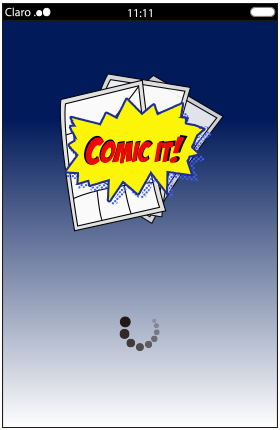
\includegraphics[width=0.4\textwidth]{demo5.jpg}
		\end{center}
	\end{frame}
	\begin{frame}
		\begin{center} 
			 
\includegraphics[width=0.4\textwidth]{demo6.jpg}
		\end{center}
	\end{frame}
	\begin{frame}
		\begin{center} 
			 
\includegraphics[width=0.4\textwidth]{demo7.jpg}
		\end{center}
	\end{frame}
	\begin{frame}
		\begin{center} 
			 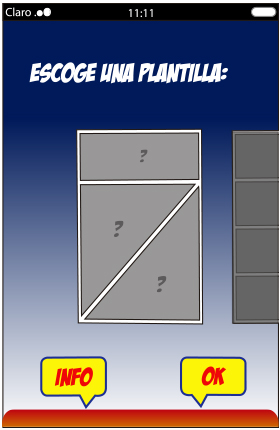
\includegraphics[width=0.4\textwidth]{demo8.jpg}
		\end{center}
	\end{frame}
	\begin{frame}
		\begin{center} 
			 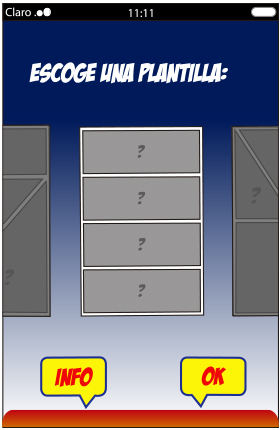
\includegraphics[width=0.4\textwidth]{demo9.jpg}
		\end{center}
	\end{frame}
	\begin{frame}
		\begin{center} 
			 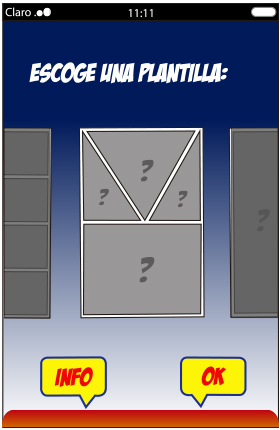
\includegraphics[width=0.4\textwidth]{demo10.jpg}
		\end{center}
	\end{frame}
	\begin{frame}
		\begin{center} 
			 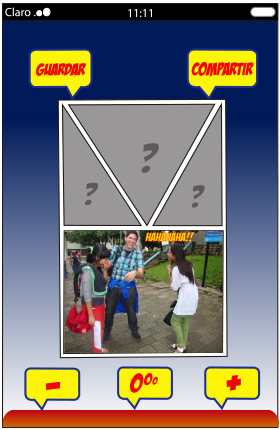
\includegraphics[width=0.4\textwidth]{demo11.jpg}
		\end{center}
	\end{frame}
	\begin{frame}
		\begin{center} 
			 
\includegraphics[width=0.8\textwidth]{gracias.jpg}
		\end{center}
	\end{frame}
\end{document}

